\documentclass[12pt,a4paper]{article}
\usepackage{iftex}
\ifPDFTeX
    \usepackage[utf8]{inputenc}
    \usepackage[T1]{fontenc}
    \usepackage{CJKutf8}
\else
    \usepackage[UTF8]{ctex}
\fi
\usepackage[margin=2.2cm]{geometry}
\usepackage{graphicx}
\usepackage{booktabs}
\usepackage{longtable}
\usepackage{array}
\usepackage{float}
\usepackage{subcaption}
\usepackage{siunitx}
\usepackage{enumitem}
\usepackage{hyperref}
\usepackage{xcolor}
\usepackage{setspace}
\usepackage{titlesec}
\usepackage{fancyhdr}
\usepackage{multirow}
\usepackage{listings}

\hypersetup{colorlinks=true,linkcolor=blue,urlcolor=blue,citecolor=blue}
\setlength{\parindent}{2em}
\setlength{\parskip}{0.35em}
\onehalfspacing
\setlist[itemize]{leftmargin=2em,itemsep=0.2em,topsep=0.3em}
\setlist[enumerate]{leftmargin=2.2em,itemsep=0.2em,topsep=0.3em}
\captionsetup{font=small,labelfont=bf}
\sisetup{round-mode=places,round-precision=2}
\lstdefinestyle{matlabstyle}{
    language=Matlab,
    basicstyle=\ttfamily\small,
    keywordstyle=\color{blue!70!black},
    commentstyle=\color{green!40!black},
    stringstyle=\color{orange!60!black},
    numbers=left,
    numberstyle=\scriptsize\color{gray},
    stepnumber=1,
    numbersep=8pt,
    frame=single,
    rulecolor=\color{black!20},
    breaklines=true,
    showstringspaces=false,
    tabsize=4
}
\lstset{style=matlabstyle}

\titleformat{\section}{\Large\bfseries}{\thesection}{0.8em}{}
\titleformat{\subsection}{\large\bfseries}{\thesubsection}{0.6em}{}
\titleformat{\subsubsection}{\normalsize\bfseries}{\thesubsubsection}{0.6em}{}

\pagestyle{fancy}
\fancyhf{}
\fancyhead[L]{语音信号处理实验二报告}
\fancyhead[R]{\thepage}

\begin{document}
\ifPDFTeX\begin{CJK*}{UTF8}{gbsn}\fi

\begin{center}
    {\Huge\bfseries 语音信号处理实验二报告\par}
    \vspace{0.8em}
    {\large 胡伟毅\quad 12313505\par}
\end{center}

\vspace{1.2em}

\section{实验目的}
\begin{enumerate}
    \item 掌握 MATLAB 语音录制与音频读写（\texttt{audiorecorder}/\texttt{audioread}/\texttt{audiowrite}）。
    \item 掌握句子级语音分段与 ARPAbet 音素标注方法。
    \item 学习使用 Praat 进行元音 Formant 提取与可视化分析。
    \item 设计并验证线性相位 FIR 高通滤波器，抑制 DC 与 60 Hz 干扰。
\end{enumerate}

\section{Problem 1：分段标注与可懂度测试}

\subsection{题目要求逐条对应}
\begin{table}[H]
\centering
\begin{tabular}{>{\centering\arraybackslash}p{1.3cm}p{9.8cm}p{3.2cm}}
\toprule
要求编号 & 题目要求 & 本文对应位置 \\
\midrule
1 & 用 ARPAbet 写出 ``Oak is strong and also gives shade'' 的音标转写 & \S2.2 \\
2 & 用 plotting/listening 对 \texttt{s5.wav} 分段并标注（含首尾静音、可能中间静音） & \S2.3--\S2.4 \\
3 & 将所有元音区间置零并试听 & \S2.5 \\
4 & 将所有辅音区间置零并试听 & \S2.6 \\
5 & 判断两种修改语音哪一种更可懂 & \S2.7 \\
\bottomrule
\end{tabular}
\end{table}

\subsection{ARPAbet 转写（对应要求1）}
目标句子：\textit{Oak is strong and also gives shade.}

ARPAbet 转写结果：
\begin{center}
\texttt{OW K | IH Z | S T R AO NG | AE N D | AO L S OW | G IH V Z | SH EY D}
\end{center}

\subsection{分段标注方法（对应要求2）}
采用波形可视化与试听结合的方式，对 \texttt{s5.wav} 进行句子级音素分段与标签标注。分段结果保存为 \texttt{problem1\_segments.csv}，共 25 段（含首尾静音）。

\subsection{分段标注结果表（对应要求2）}
\begin{center}
\small
\begin{longtable}{>{\centering\arraybackslash}p{0.8cm}>{\centering\arraybackslash}p{3.2cm}>{\centering\arraybackslash}p{1.4cm}>{\centering\arraybackslash}p{1.8cm}>{\centering\arraybackslash}p{2cm}}
\caption{Problem 1 分段与标注结果（段间相差一个采样周期）}\\
\toprule
段号 & 时间区间(s) & 标签 & 类型 & 单词 \\
\midrule
\endfirsthead
\toprule
段号 & 时间区间(s) & 标签 & 类型 & 单词 \\
\midrule
\endhead
1 & 0.000000 -- 0.159750 & SIL & silence & - \\
2 & 0.159875 -- 0.279750 & OW & vowel & Oak \\
3 & 0.279875 -- 0.344750 & K & consonant & Oak \\
4 & 0.344875 -- 0.579750 & IH & vowel & is \\
5 & 0.579875 -- 0.724750 & Z & consonant & is \\
6 & 0.724875 -- 0.769750 & S & consonant & strong \\
7 & 0.769875 -- 0.784750 & T & consonant & strong \\
8 & 0.784875 -- 0.804750 & R & consonant & strong \\
9 & 0.804875 -- 0.864750 & AO & vowel & strong \\
10 & 0.864875 -- 1.194750 & NG & consonant & strong \\
11 & 1.194875 -- 1.214750 & AE & vowel & and \\
12 & 1.214875 -- 1.274750 & N & consonant & and \\
13 & 1.274875 -- 1.319750 & D & consonant & and \\
14 & 1.319875 -- 1.369750 & AO & vowel & also \\
15 & 1.369875 -- 1.499750 & L & consonant & also \\
16 & 1.499875 -- 1.589750 & S & consonant & also \\
17 & 1.589875 -- 1.684750 & OW & vowel & also \\
18 & 1.684875 -- 1.779750 & G & consonant & gives \\
19 & 1.779875 -- 1.884750 & IH & vowel & gives \\
20 & 1.884875 -- 1.934750 & V & consonant & gives \\
21 & 1.934875 -- 1.999750 & Z & consonant & gives \\
22 & 1.999875 -- 2.094750 & SH & consonant & shade \\
23 & 2.094875 -- 2.349750 & EY & vowel & shade \\
24 & 2.349875 -- 2.429750 & D & consonant & shade \\
25 & 2.429875 -- 2.999875 & SIL & silence & - \\
\bottomrule
\end{longtable}
\end{center}

\begin{figure}[H]
    \centering
    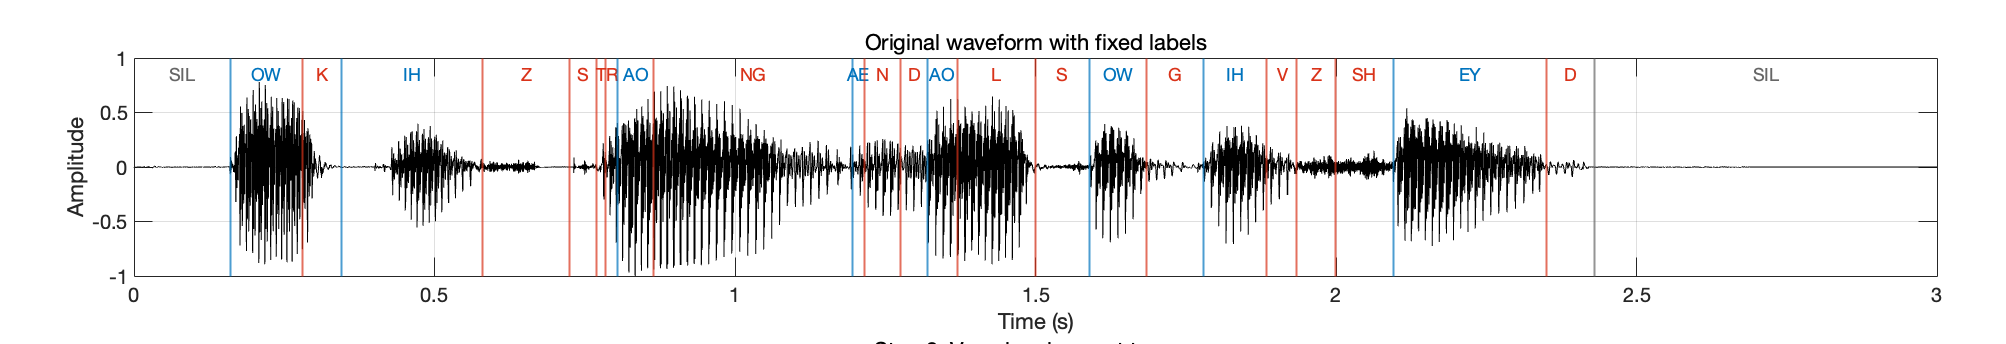
\includegraphics[width=0.85\textwidth]{figures/fig01.png}
    \caption{Problem 1 分段主图（蓝色元音、红色辅音）}
\end{figure}

\subsection{元音置零结果（对应要求3）}
将标注为元音（vowel）的样本区间置零，生成输出文件：\texttt{problem1\_no\_vowels.wav}。

\begin{figure}[H]
    \centering
    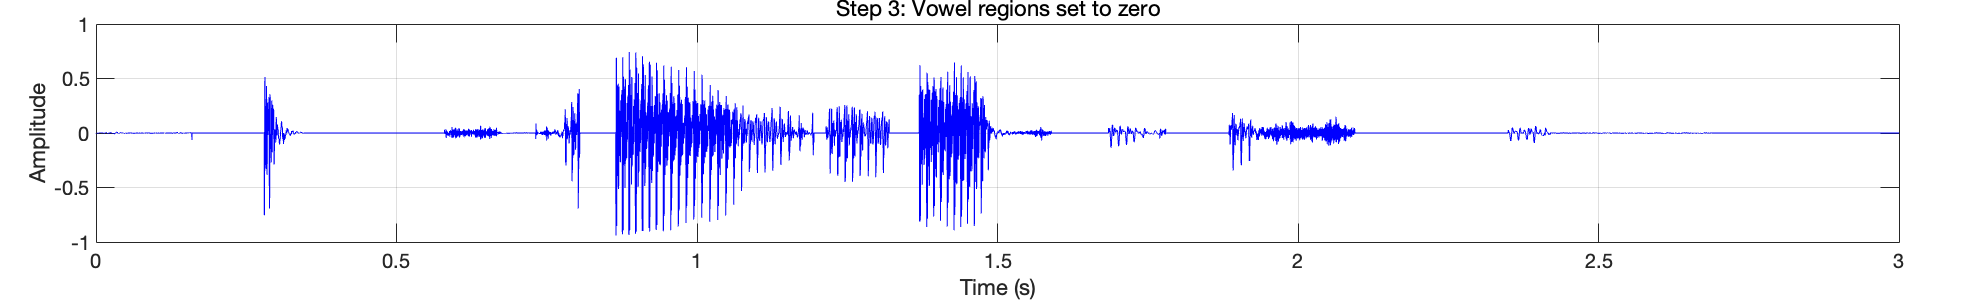
\includegraphics[width=0.8\textwidth]{figures/fig02.png}
    \caption{元音置零后的波形结果}
\end{figure}

\subsection{辅音置零结果（对应要求4）}
将标注为辅音（consonant）的样本区间置零，生成输出文件：\texttt{problem1\_no\_consonants.wav}。

\begin{figure}[H]
    \centering
    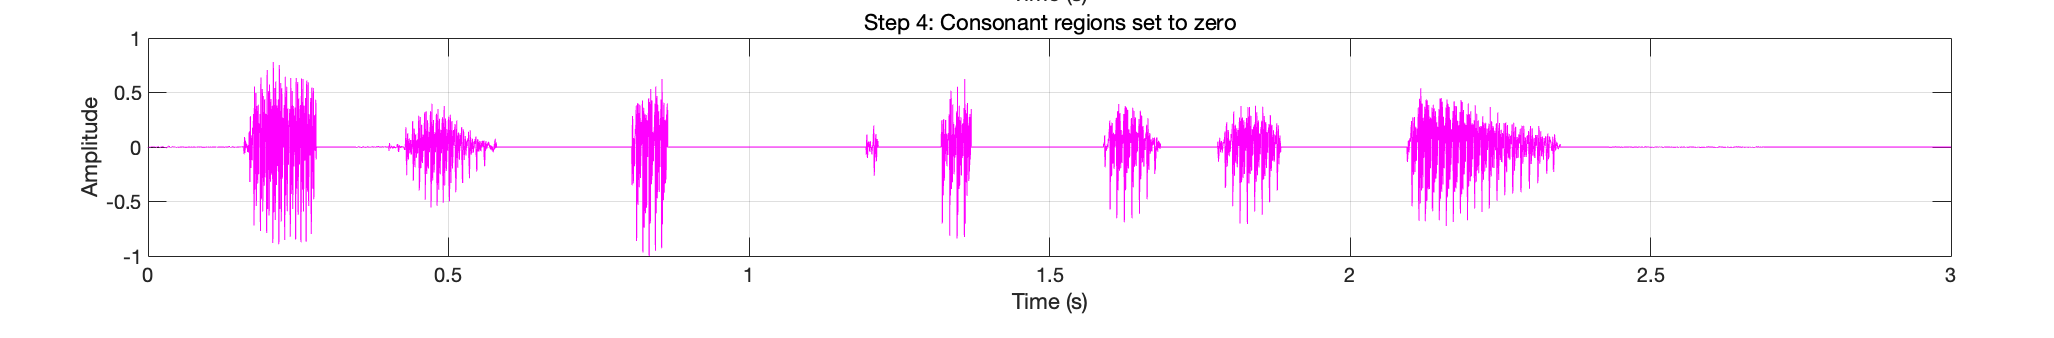
\includegraphics[width=0.8\textwidth]{figures/fig03.png}
    \caption{辅音置零后的波形结果}
\end{figure}

\subsection{可懂度判断（对应要求5）}
两种处理后语音都明显降低可懂度。对比发现，元音置零后仍能较多保留单词轮廓；辅音置零后单词边界与区分信息下降更明显。说明在本实验语句中，辅音对词汇区分（可懂度）贡献更大，而元音更多承载能量与韵律信息。

\subsection{关键代码段}
\begin{lstlisting}[caption={Problem 1 固定边界与标注表输出}]
labels = {'SIL', 'OW', 'K', 'IH', 'Z', 'S', 'T', 'R', 'AO', 'NG', ...
          'AE', 'N', 'D', 'AO', 'L', 'S', 'OW', 'G', 'IH', 'V', ...
          'Z', 'SH', 'EY', 'D', 'SIL'};

boundarySec = [ ...
    0.000000, 0.159875, 0.279875, 0.344875, 0.579875, 0.724875, ...
    0.769875, 0.784875, 0.804875, 0.864875, 1.194875, 1.214875, ...
    1.274875, 1.319875, 1.369875, 1.499875, 1.589875, 1.684875, ...
    1.779875, 1.884875, 1.934875, 1.999875, 2.094875, 2.349875, ...
    2.429875, 3.000000 ...
];

segmentTable = table(segmentId, segStart, segEnd, labelCol, typeCol, wordCol, ...
    'VariableNames', {'Segment', 'Start_s', 'End_s', 'Label', 'Type', 'Word'});
writetable(segmentTable, 'problem1_segments.csv');
\end{lstlisting}

\begin{lstlisting}[caption={Problem 1 元音/辅音置零与导出}]
vowelMask = false(N, 1);
consMask = false(N, 1);
for k = 1:nSeg
    idx = bounds(k):(bounds(k+1)-1);
    if strcmp(types{k}, 'vowel')
        vowelMask(idx) = true;
    elseif strcmp(types{k}, 'consonant')
        consMask(idx) = true;
    end
end

xNoVowels = x;      xNoVowels(vowelMask) = 0;
xNoConsonants = x;  xNoConsonants(consMask) = 0;
audiowrite('problem1_no_vowels.wav', xNoVowels, fs);
audiowrite('problem1_no_consonants.wav', xNoConsonants, fs);
\end{lstlisting}

\section{Problem 2：元音录制、FFT 分析与 Praat 对比}

\subsection{题目要求逐条对应}
\begin{table}[H]
\centering
\begin{tabular}{>{\centering\arraybackslash}p{1.3cm}p{9.8cm}p{3.2cm}}
\toprule
要求编号 & 题目要求 & 本文对应位置 \\
\midrule
1 & MATLAB 中用 \texttt{audiowrite} 与 \texttt{audiorecorder} 录制 /a/ /i/ /u/ & \S3.2 \\
2 & 使用 FFT 分析录制元音频谱 & \S3.3 \\
3 & 绘制 dB 频谱并找谱包络峰值频率 & \S3.4 \\
4 & 用 Praat 重复录音和分析并展示结果 & \S3.5 \\
5 & 比较 FFT 与 Praat 提取的 formant frequencies & \S3.6--\S3.7 \\
\bottomrule
\end{tabular}
\end{table}

\subsection{MATLAB 录音与数据准备（对应要求1）}
录制参数：采样率 \SI{16}{kHz}，单通道，单次时长 \SI{1.5}{s}。
生成文件：\texttt{problem2\_a.wav}（AA）、\texttt{problem2\_i.wav}（IY）、\texttt{problem2\_u.wav}（UW）。

\subsection{FFT 分析流程（对应要求2）}
对每个元音提取中间稳态 \SI{40}{ms}，加 Hamming 窗，\texttt{nfft=8192}，计算单边 dB 频谱，并采用平滑包络提取峰值。

\subsection{dB 频谱与峰值标注（对应要求3）}
由于包络极值存在不稳定现象，本实验先参考标准共振峰位置，再在其邻域内搜索实测峰值并标注。

\begin{figure}[H]
    \centering
    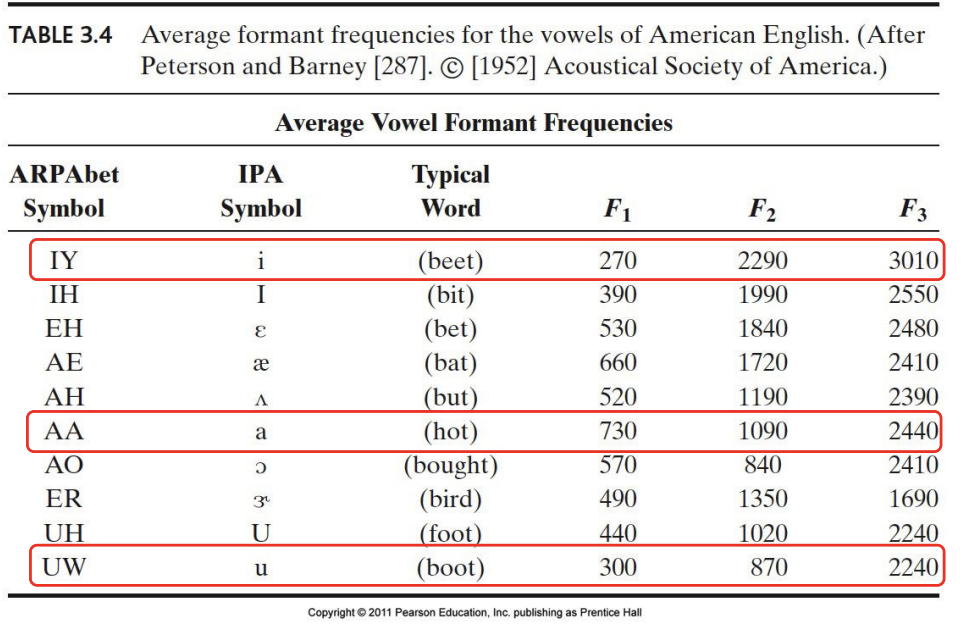
\includegraphics[width=0.78\textwidth]{figures/fig04.png}
    \caption{理论（标准）共振峰参考值}
\end{figure}

\begin{figure}[H]
    \centering
    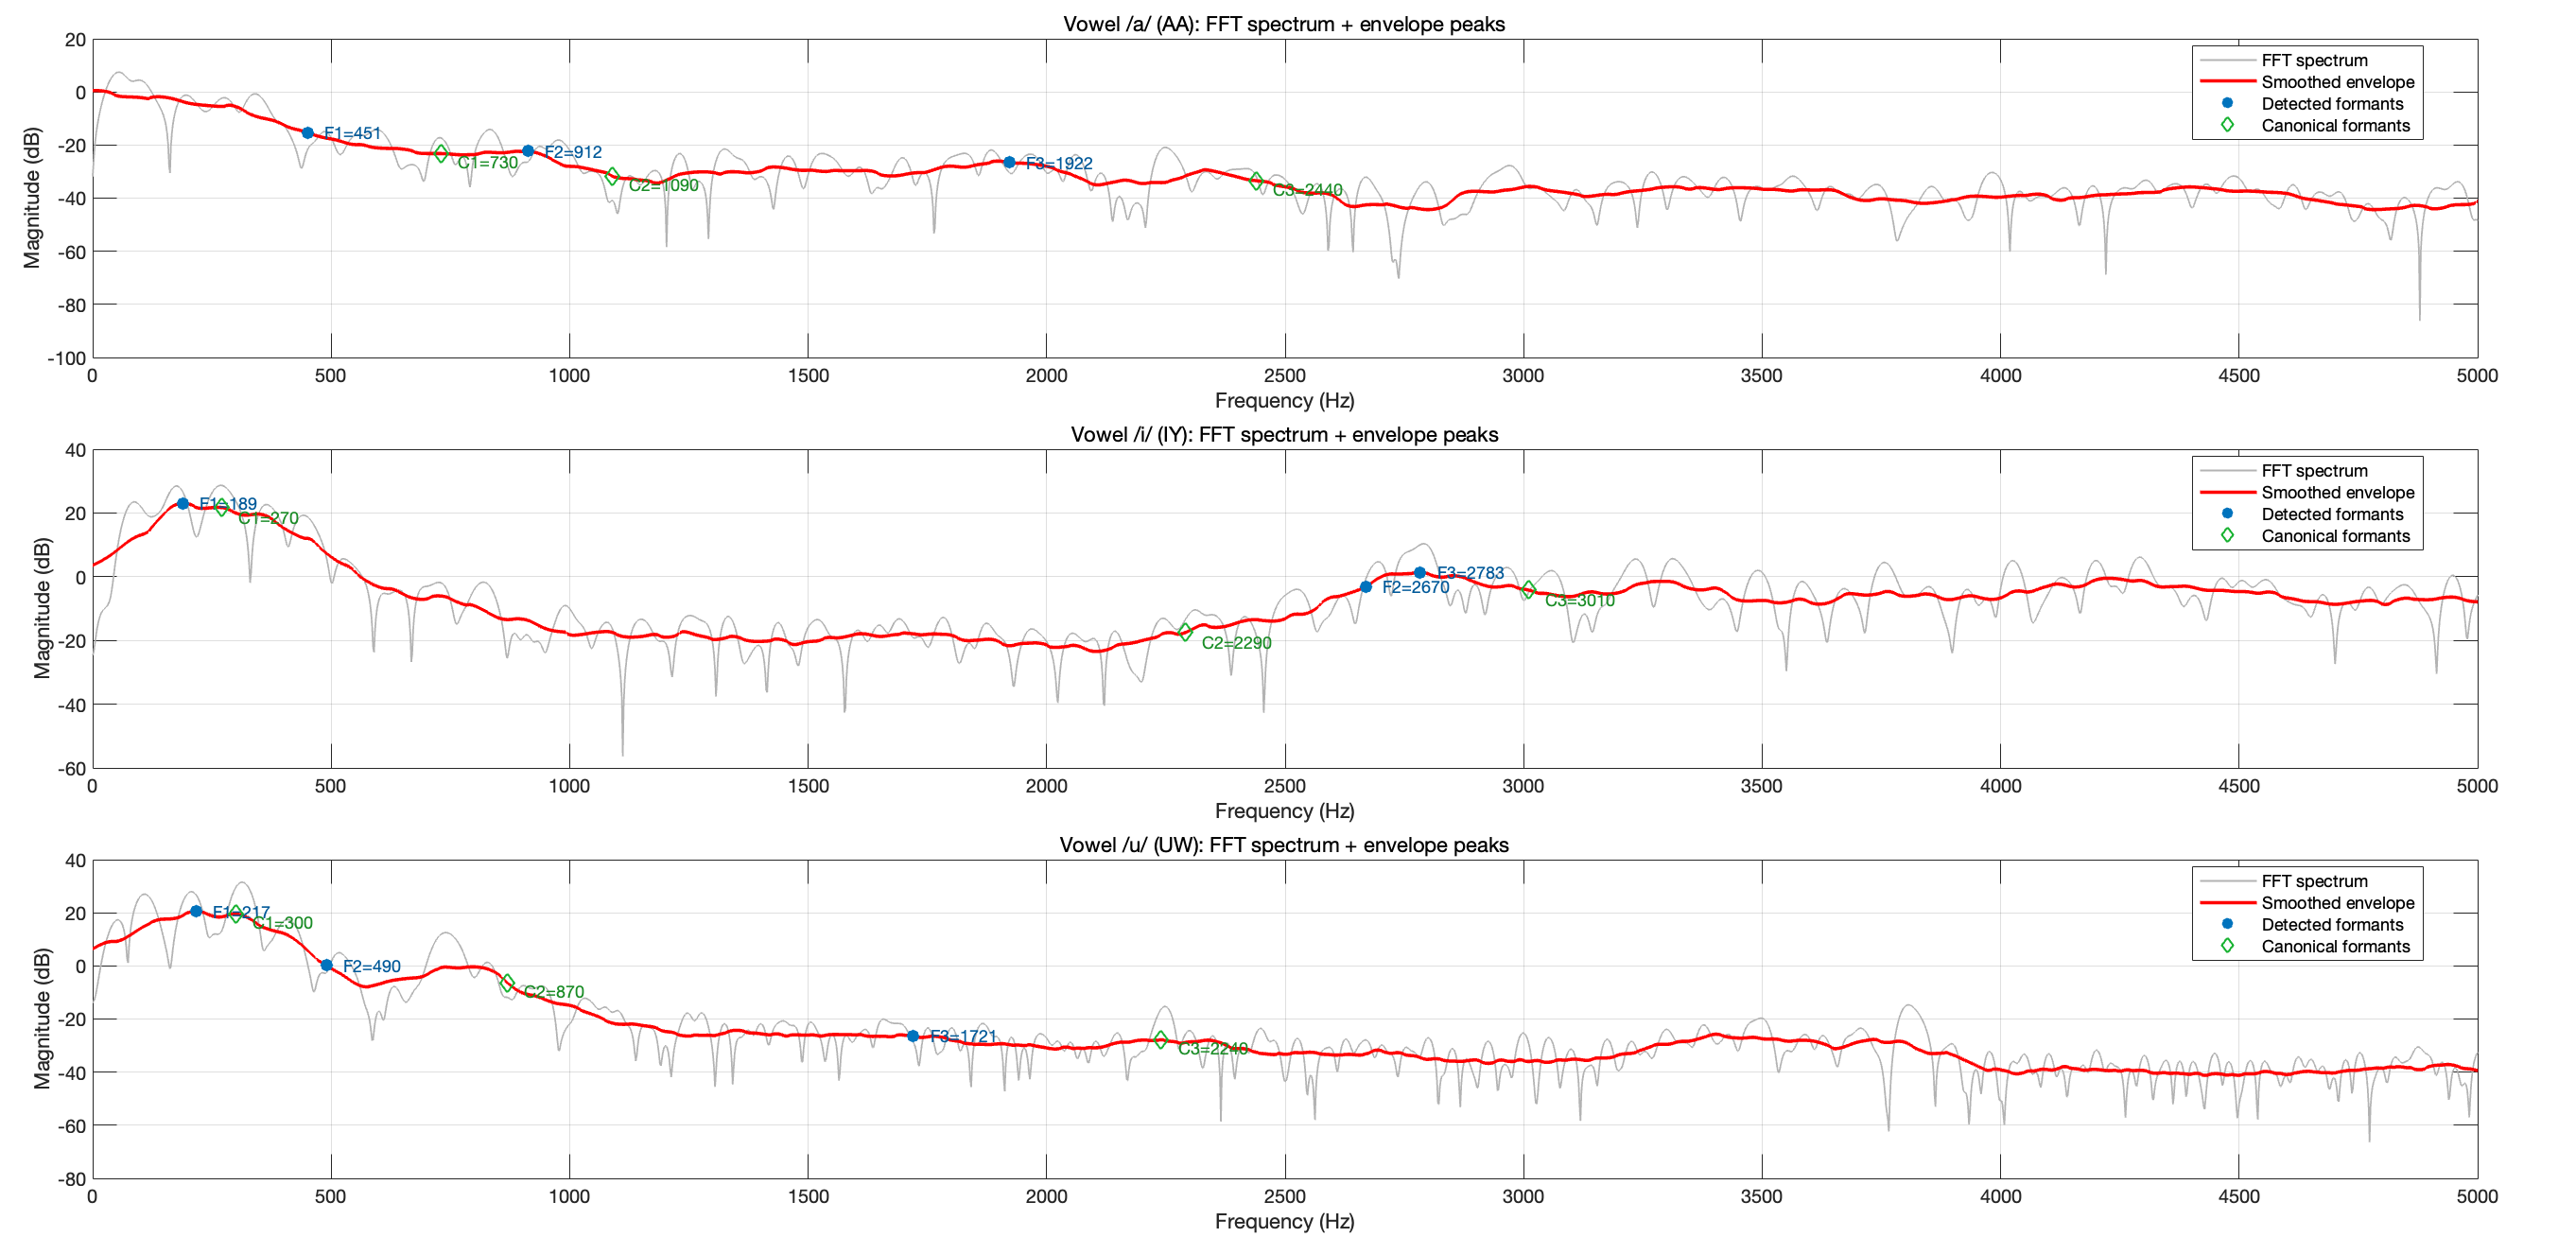
\includegraphics[width=\textwidth]{figures/fig05.png}
    \caption{三元音 FFT 频谱：灰线为 FFT，红线为平滑包络，蓝点为检测峰值，绿菱形为标准值}
\end{figure}

MATLAB（FFT）提取结果：
\begin{table}[H]
\centering
\begin{tabular}{cS[table-format=4.2]S[table-format=4.2]S[table-format=4.2]}
\toprule
元音 & {F1 (Hz)} & {F2 (Hz)} & {F3 (Hz)} \\
\midrule
AA & 451.17 & 912.11 & 1921.88 \\
IY & 189.45 & 2669.92 & 2783.20 \\
UW & 216.80 & 490.23 & 1720.70 \\
\bottomrule
\end{tabular}
\caption{MATLAB（FFT）提取的 Formant 结果}
\end{table}

\subsection{Praat 分析结果（对应要求4）}
对 AA、IY、UW 三个音分别在稳态段读取 F1/F2/F3。为节省版面，每个音标的 3 张截图排在同一行。

\begin{figure}[H]
\centering
\begin{subfigure}[t]{0.32\textwidth}
    \centering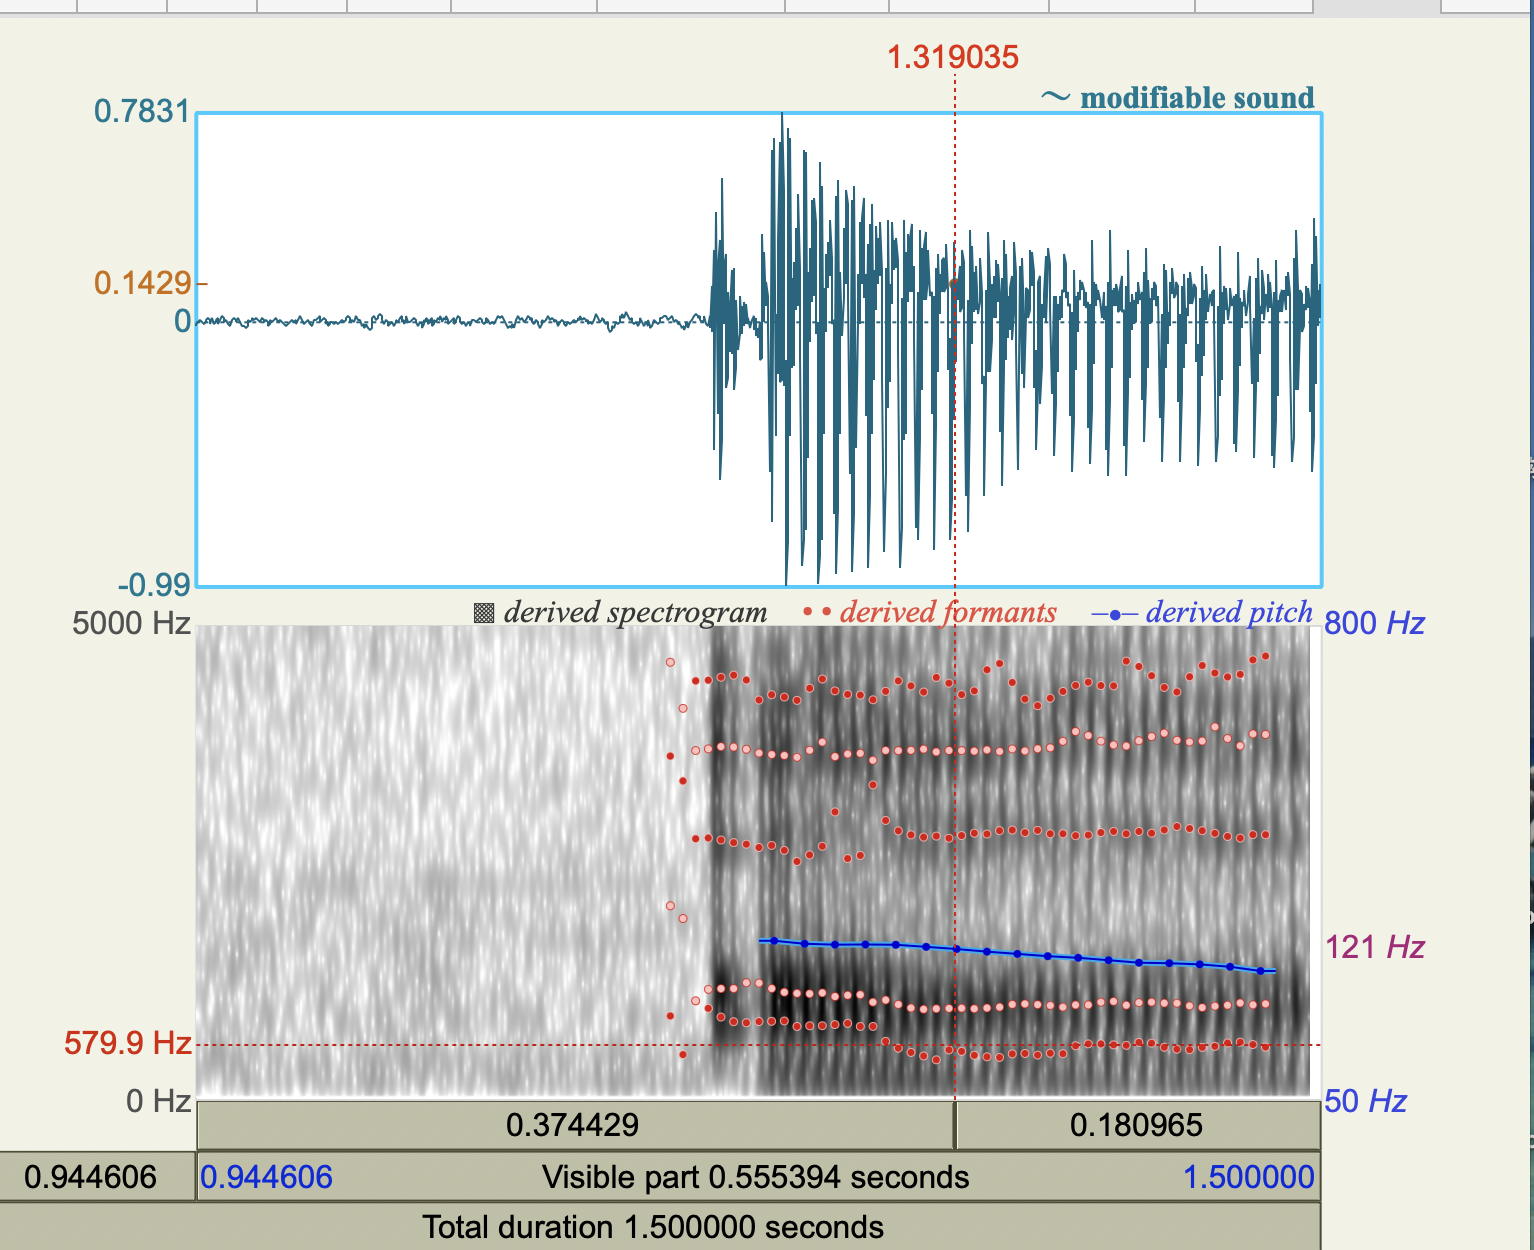
\includegraphics[width=\textwidth]{figures/fig06.png}
\end{subfigure}
\hfill
\begin{subfigure}[t]{0.32\textwidth}
    \centering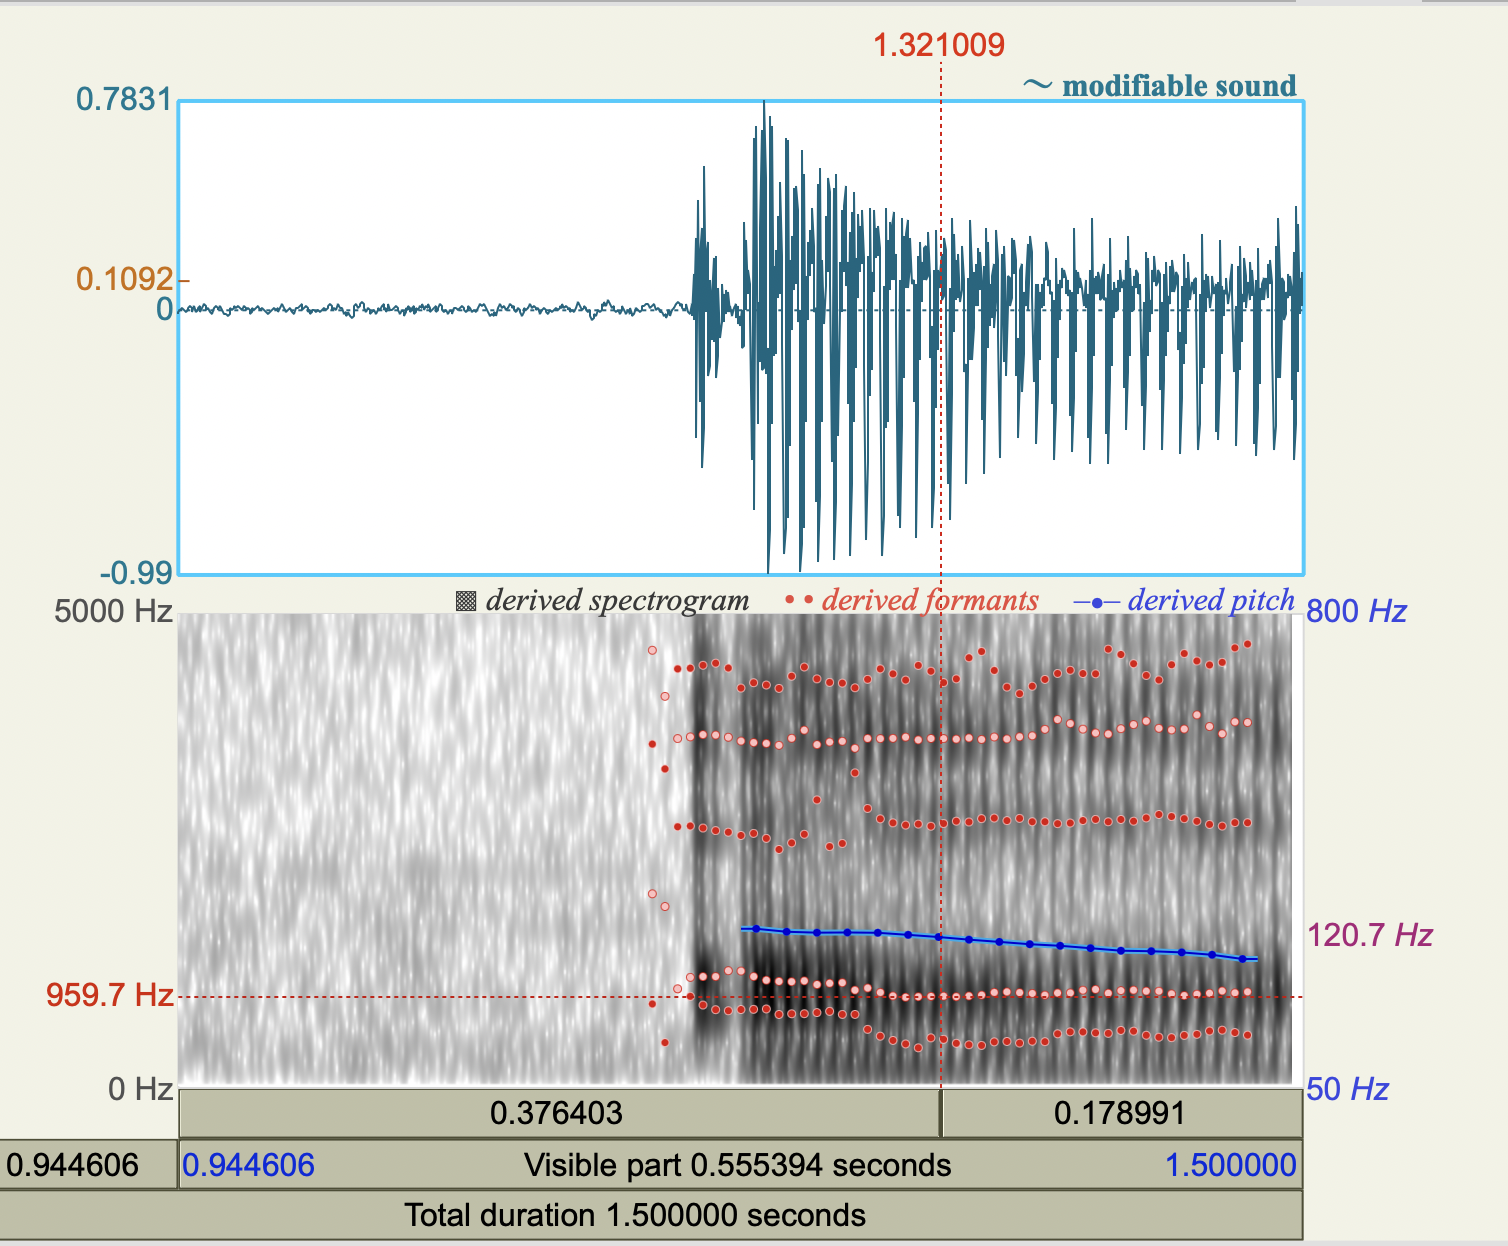
\includegraphics[width=\textwidth]{figures/fig07.png}
\end{subfigure}
\hfill
\begin{subfigure}[t]{0.32\textwidth}
    \centering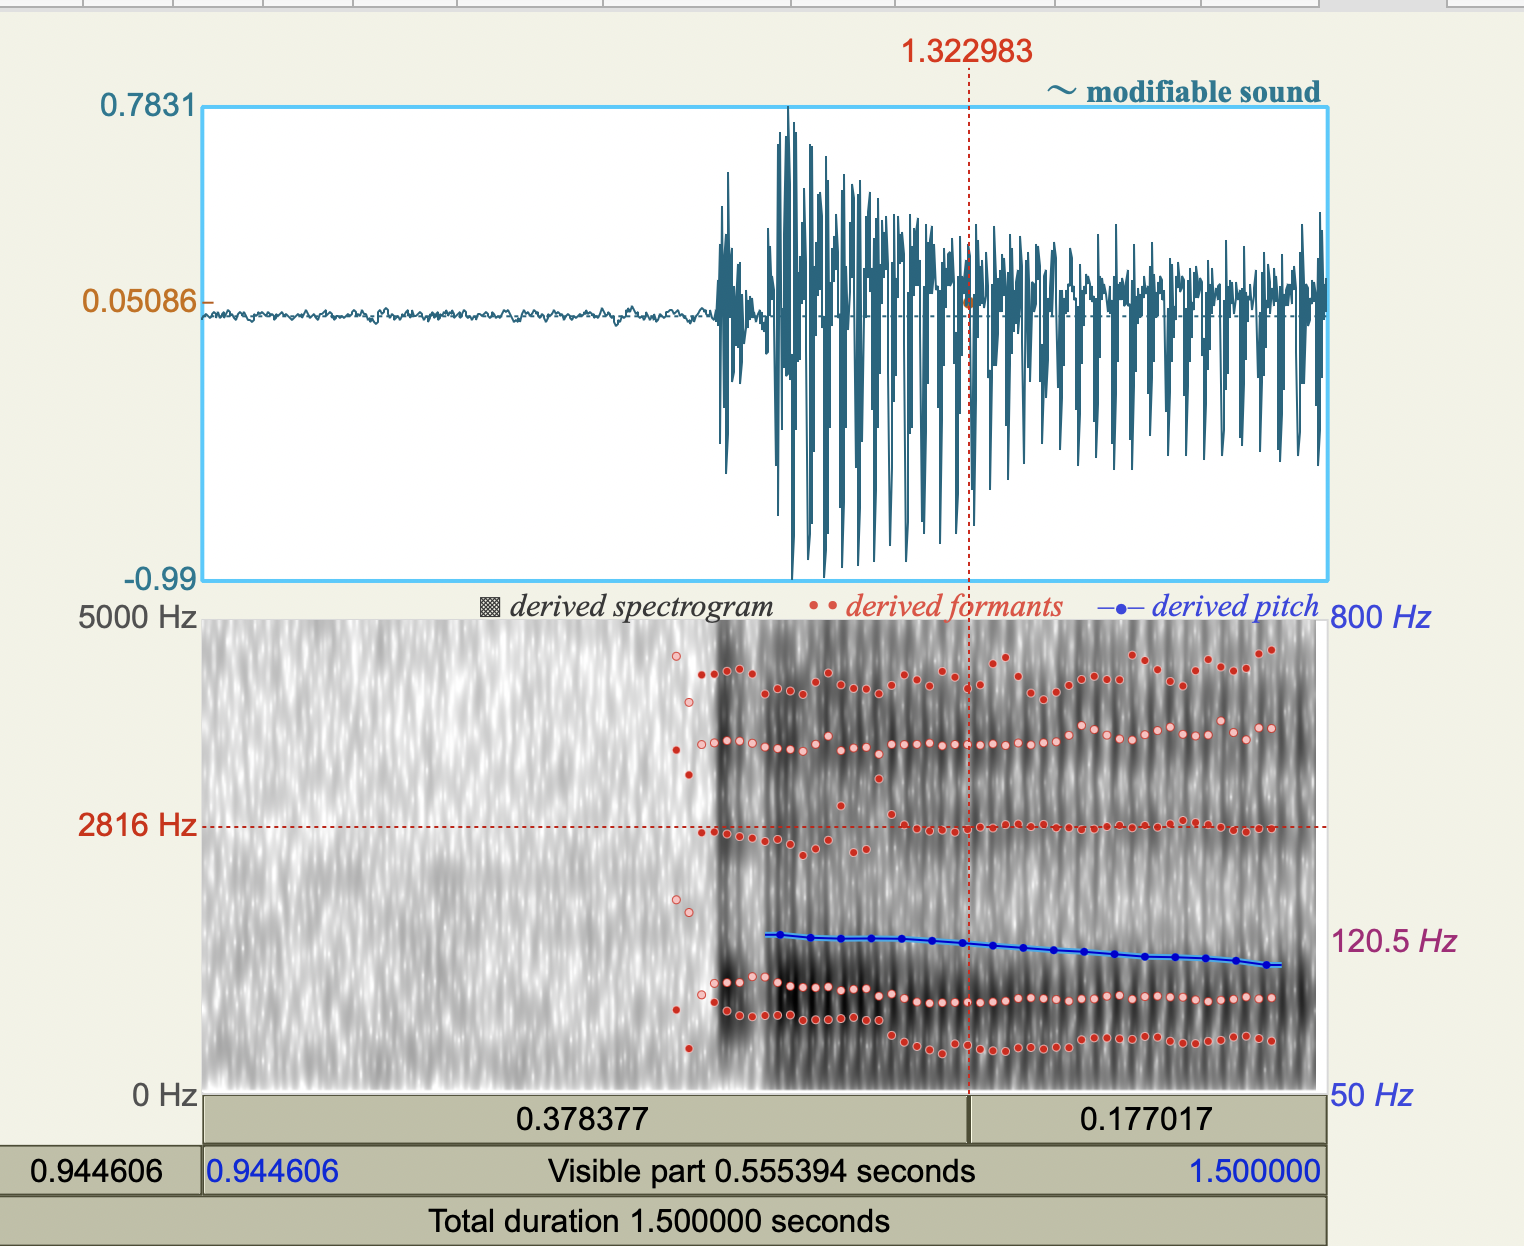
\includegraphics[width=\textwidth]{figures/fig08.png}
\end{subfigure}
\caption{Praat：AA（/a/）三次读数截图（同一行）}
\end{figure}

\begin{figure}[H]
\centering
\begin{subfigure}[t]{0.32\textwidth}
    \centering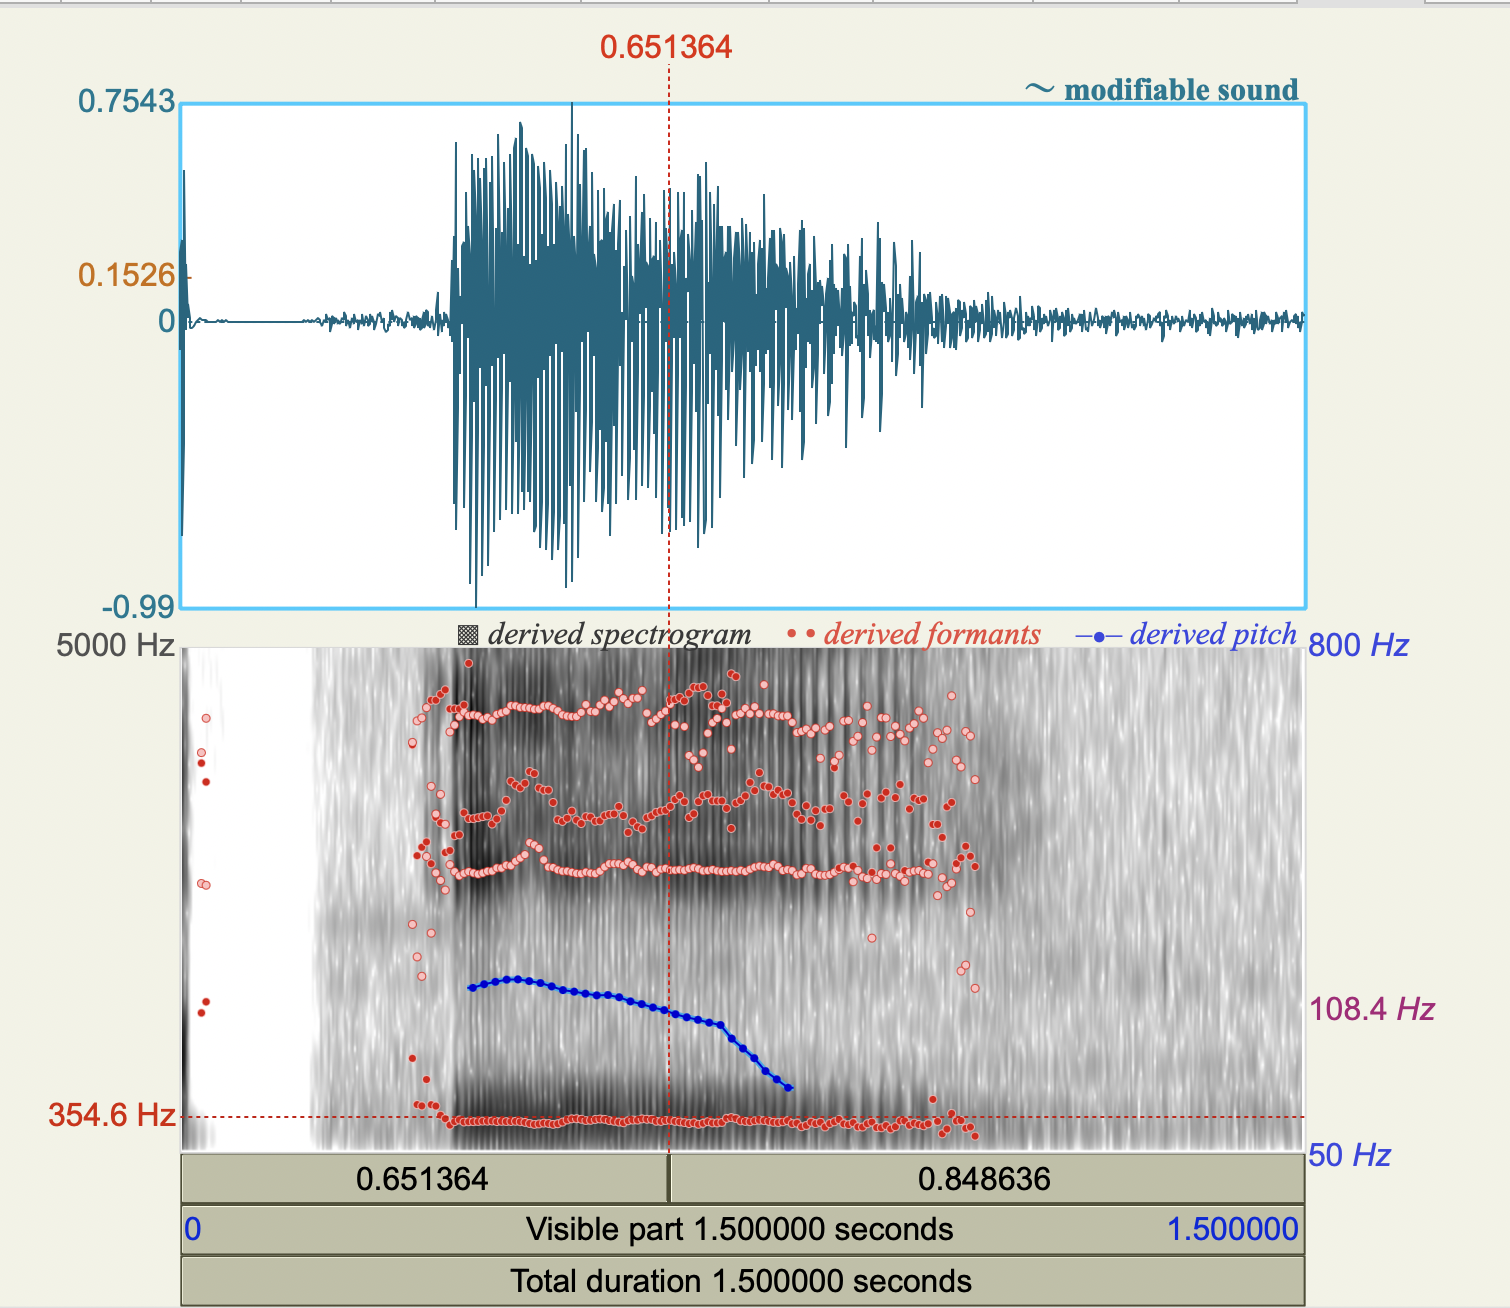
\includegraphics[width=\textwidth]{figures/fig09.png}
\end{subfigure}
\hfill
\begin{subfigure}[t]{0.32\textwidth}
    \centering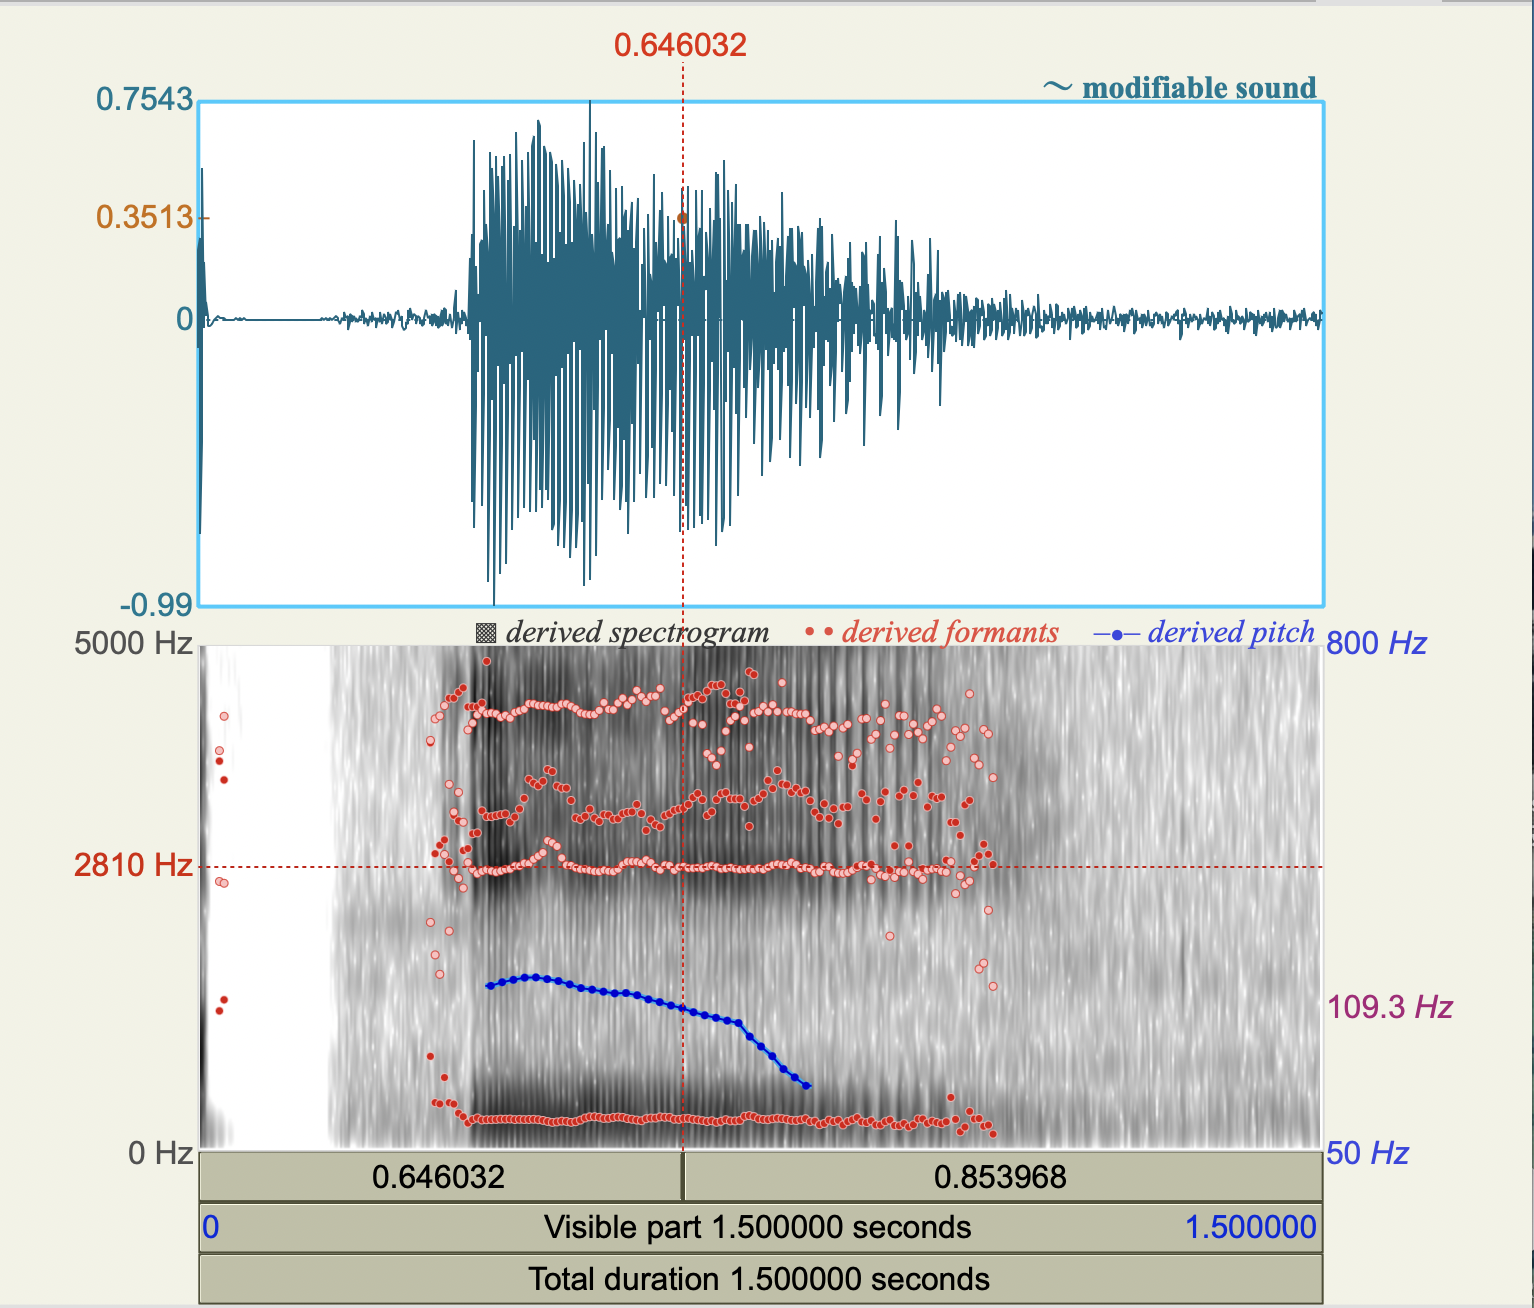
\includegraphics[width=\textwidth]{figures/fig10.png}
\end{subfigure}
\hfill
\begin{subfigure}[t]{0.32\textwidth}
    \centering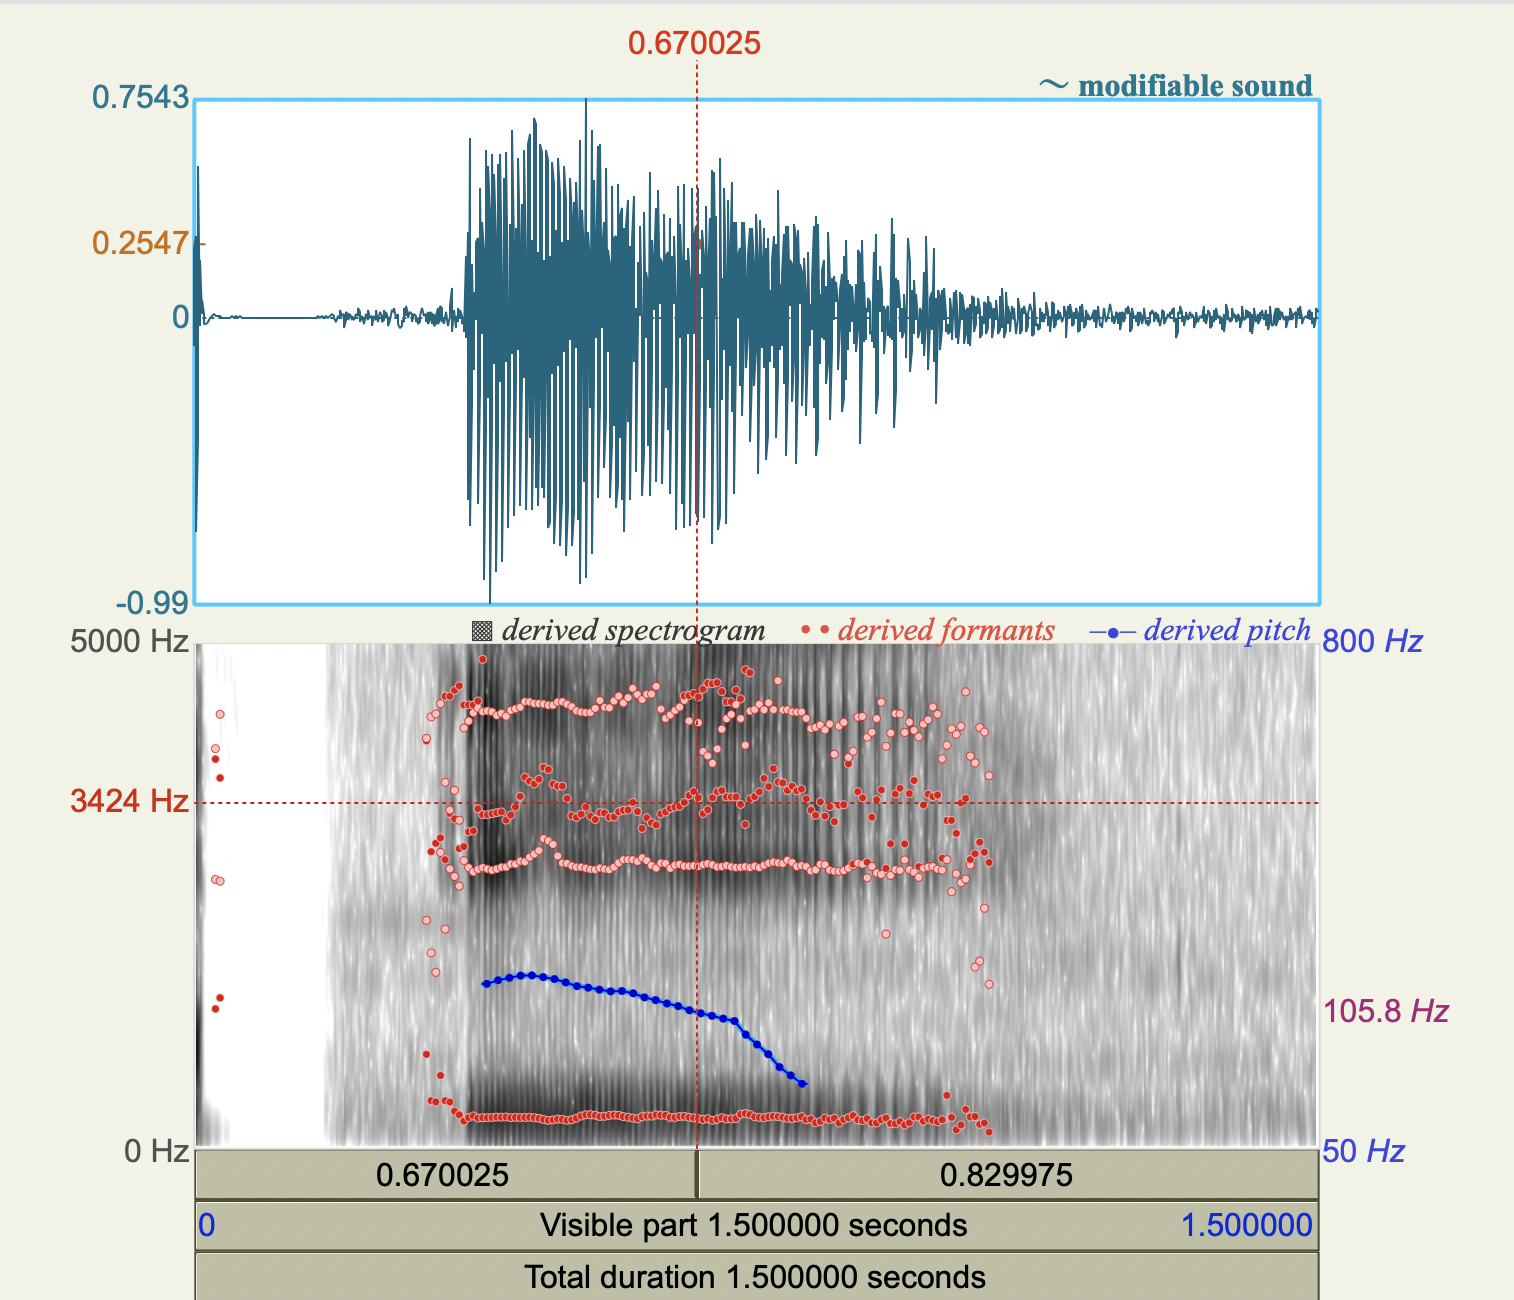
\includegraphics[width=\textwidth]{figures/fig11.png}
\end{subfigure}
\caption{Praat：IY（/i/）三次读数截图（同一行）}
\end{figure}

\begin{figure}[H]
\centering
\begin{subfigure}[t]{0.32\textwidth}
    \centering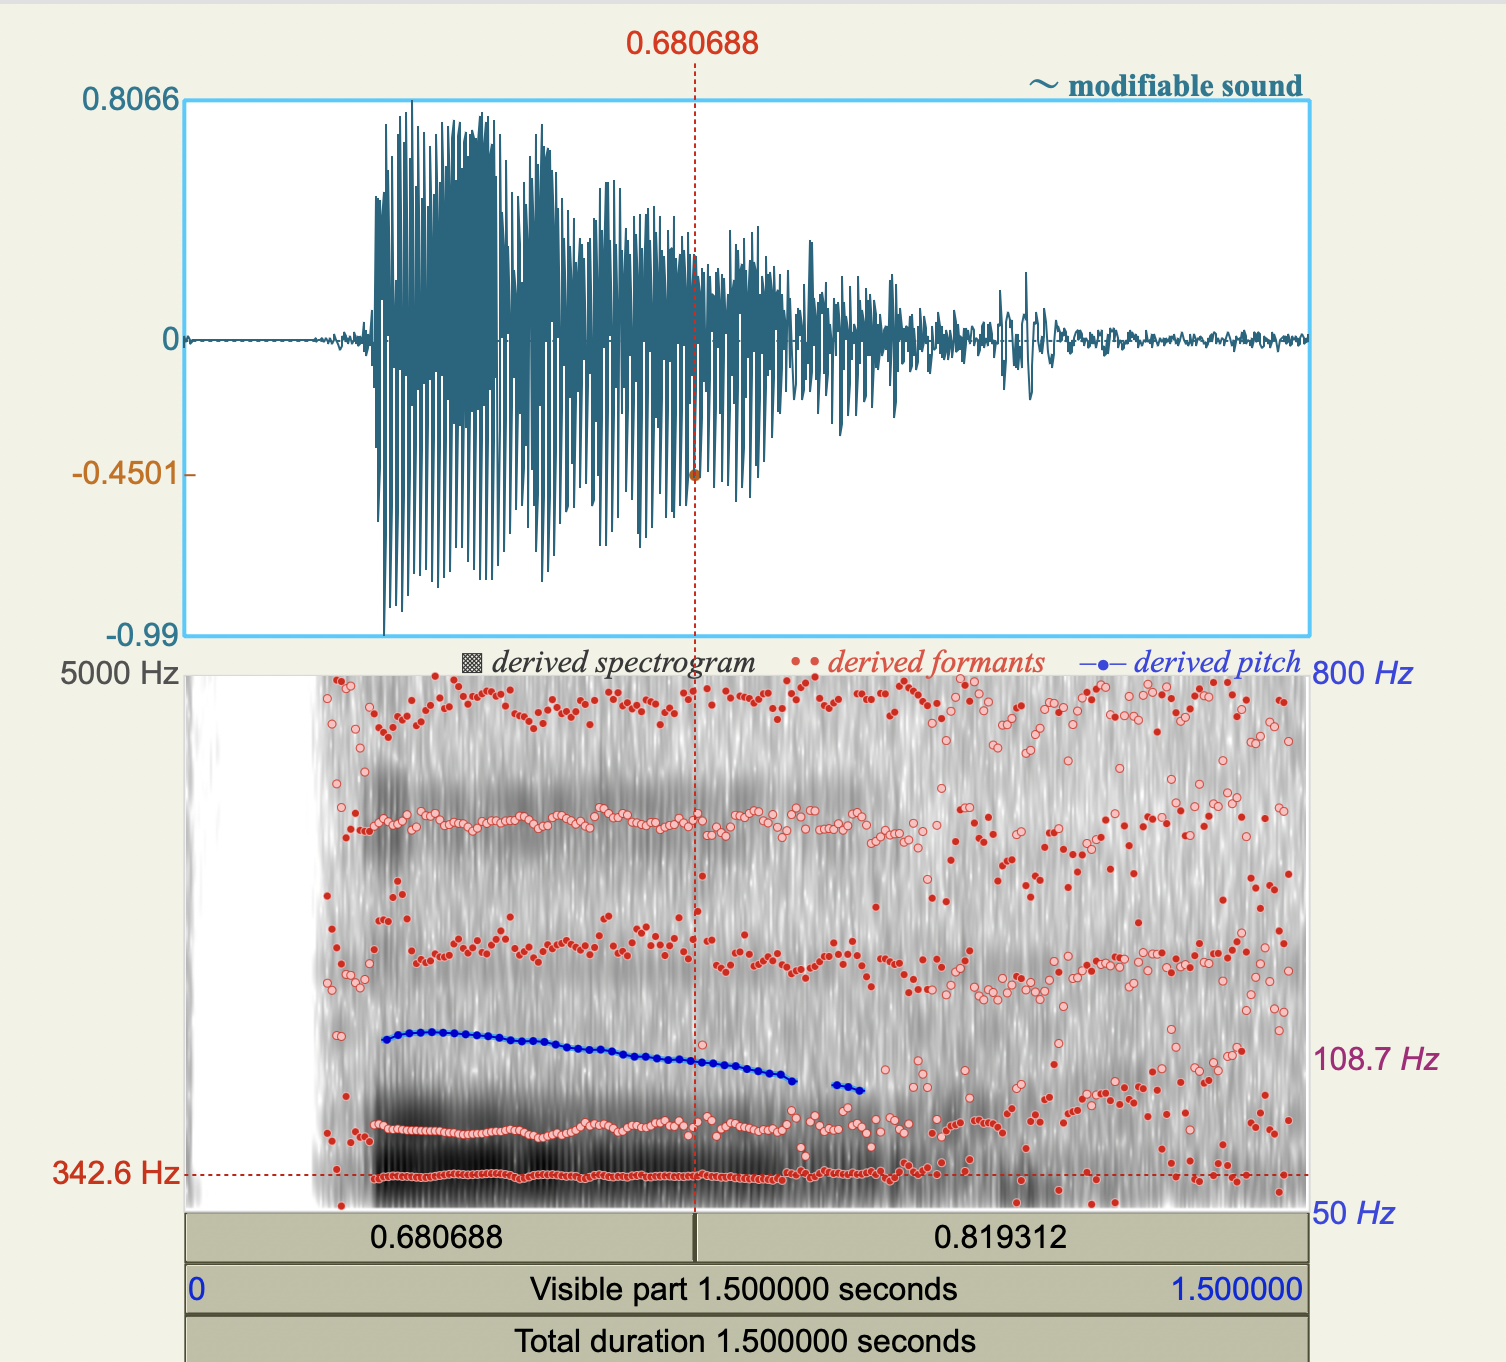
\includegraphics[width=\textwidth]{figures/fig12.png}
\end{subfigure}
\hfill
\begin{subfigure}[t]{0.32\textwidth}
    \centering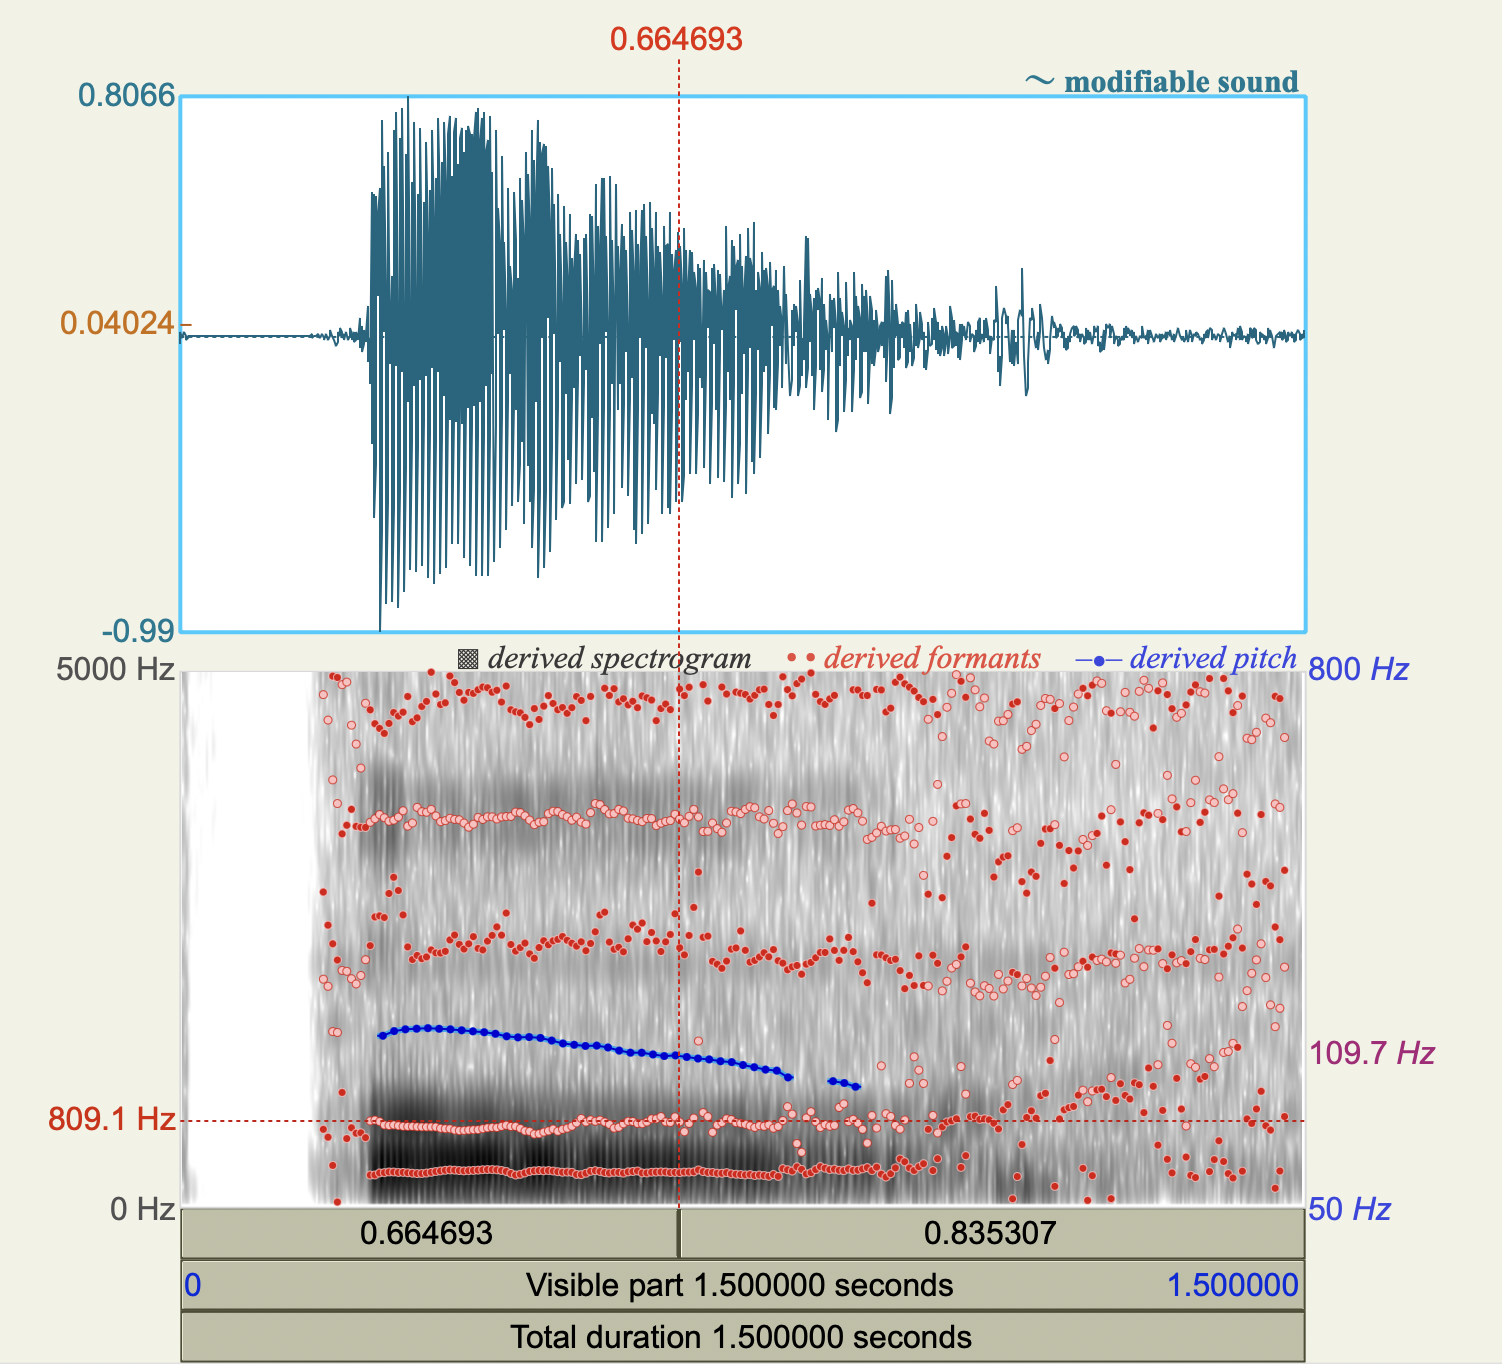
\includegraphics[width=\textwidth]{figures/fig13.png}
\end{subfigure}
\hfill
\begin{subfigure}[t]{0.32\textwidth}
    \centering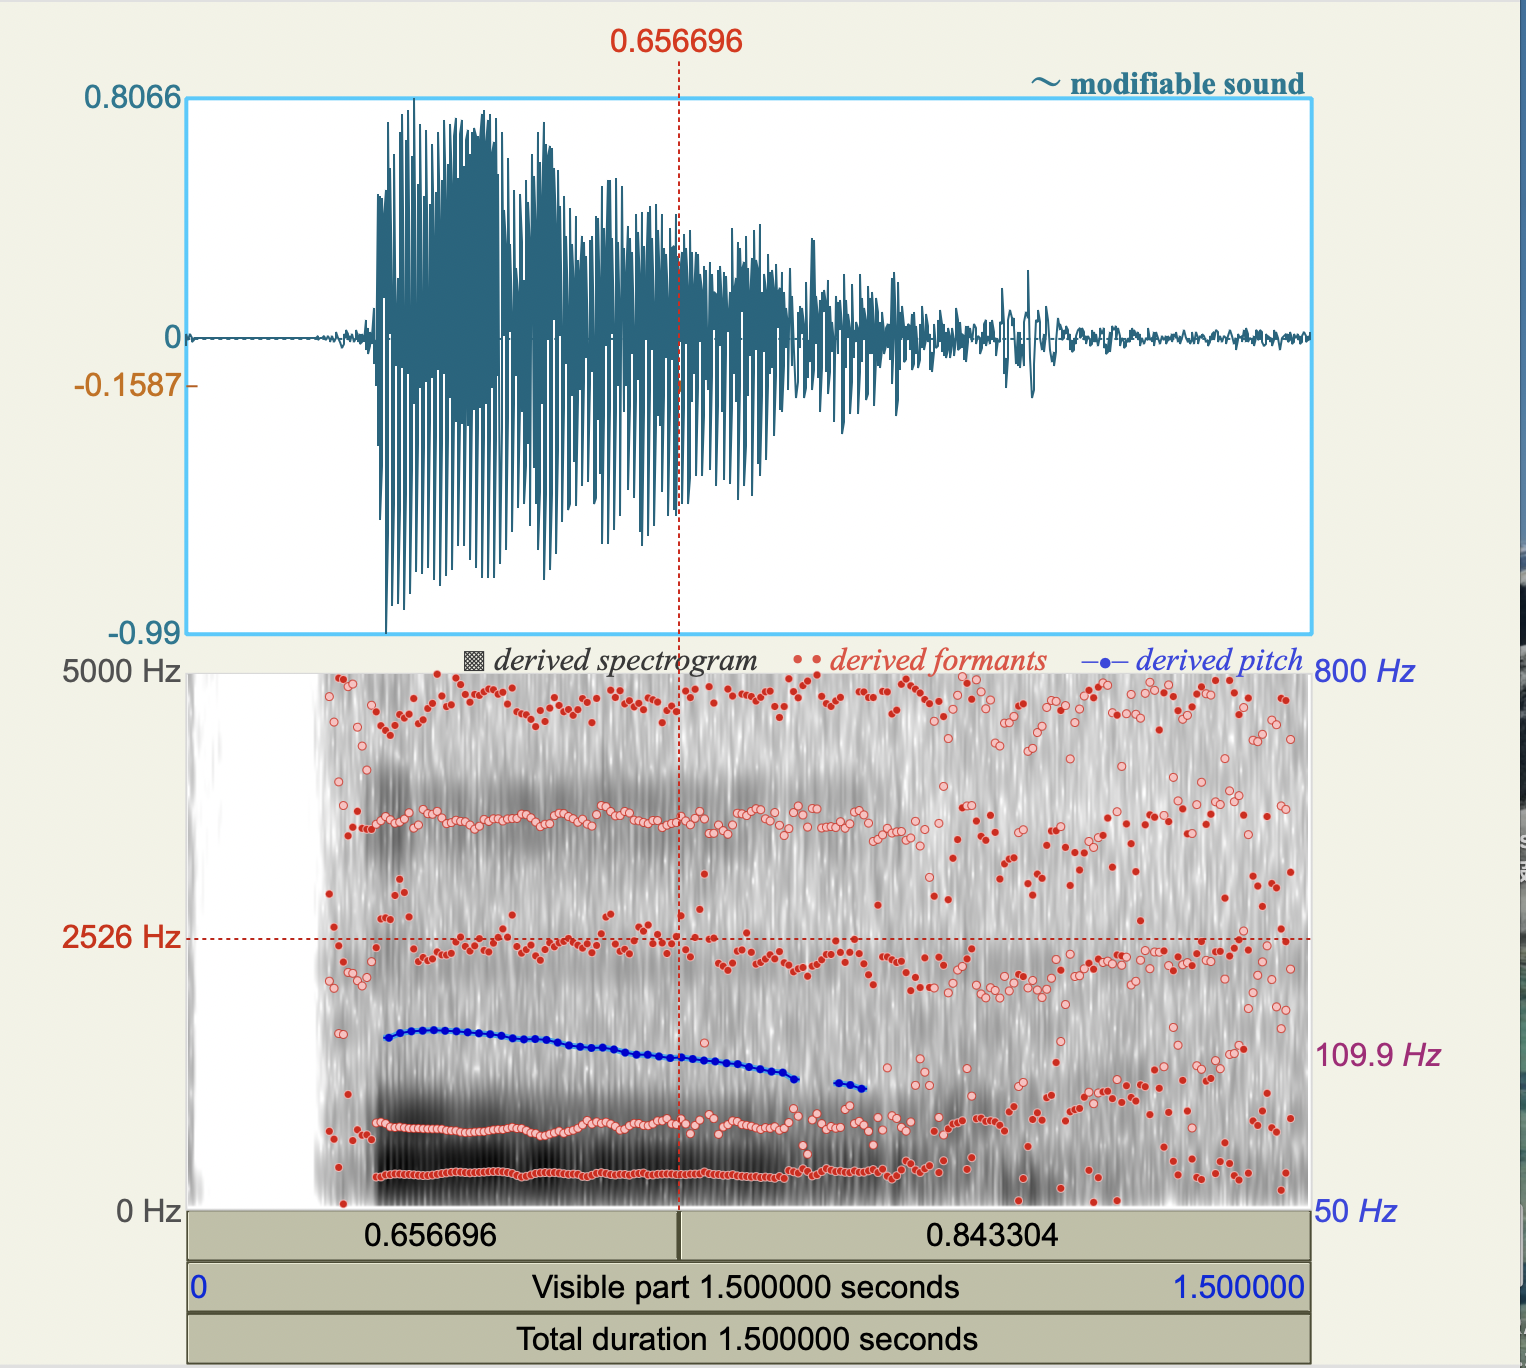
\includegraphics[width=\textwidth]{figures/fig14.png}
\end{subfigure}
\caption{Praat：UW（/u/）三次读数截图（同一行）}
\end{figure}

\begin{table}[H]
\centering
\begin{tabular}{cS[table-format=4.1]S[table-format=4.1]S[table-format=4.1]}
\toprule
元音 & {F1 (Hz)} & {F2 (Hz)} & {F3 (Hz)} \\
\midrule
AA & 579.9 & 959.7 & 2816.0 \\
IY & 354.6 & 2810.0 & 3424.0 \\
UW & 342.6 & 809.1 & 2526.0 \\
\bottomrule
\end{tabular}
\caption{Praat 提取的 Formant 结果}
\end{table}

\subsection{FFT 与 Praat 对比（对应要求5）}
\begin{table}[H]
\centering
\small
\begin{tabular}{c|S[table-format=4.2]S[table-format=4.2]S[table-format=+4.2]|S[table-format=4.2]S[table-format=4.2]S[table-format=+4.2]|S[table-format=4.2]S[table-format=4.2]S[table-format=+4.2]}
\toprule
\multirow{2}{*}{元音} & \multicolumn{3}{c|}{F1} & \multicolumn{3}{c|}{F2} & \multicolumn{3}{c}{F3} \\
 & {FFT} & {Praat} & {$\Delta$} & {FFT} & {Praat} & {$\Delta$} & {FFT} & {Praat} & {$\Delta$} \\
\midrule
AA & 451.17 & 579.90 & -128.73 & 912.11 & 959.70 & -47.59 & 1921.88 & 2816.00 & -894.12 \\
IY & 189.45 & 354.60 & -165.15 & 2669.92 & 2810.00 & -140.08 & 2783.20 & 3424.00 & -640.80 \\
UW & 216.80 & 342.60 & -125.80 & 490.23 & 809.10 & -318.87 & 1720.70 & 2526.00 & -805.30 \\
\bottomrule
\end{tabular}
\caption{FFT 与 Praat 结果对比（$\Delta=\mathrm{FFT}-\mathrm{Praat}$）}
\end{table}

\subsection{与标准值对比与分析}
标准参考值：AA=[730,1090,2440]，IY=[270,2290,3010]，UW=[300,870,2240]（单位：Hz）。

\begin{table}[H]
\centering
\small
\begin{tabular}{c|S[table-format=+4.2]S[table-format=+4.2]|S[table-format=+4.2]S[table-format=+4.2]|S[table-format=+4.2]S[table-format=+4.2]}
\toprule
\multirow{2}{*}{元音} & \multicolumn{2}{c|}{$\Delta$F1 (实测-标准)} & \multicolumn{2}{c|}{$\Delta$F2 (实测-标准)} & \multicolumn{2}{c}{$\Delta$F3 (实测-标准)} \\
 & {FFT} & {Praat} & {FFT} & {Praat} & {FFT} & {Praat} \\
\midrule
AA & -278.83 & -150.10 & -177.89 & -130.30 & -518.12 & +376.00 \\
IY & -80.55 & +84.60 & +379.92 & +520.00 & -226.80 & +414.00 \\
UW & -83.20 & +42.60 & -379.77 & -60.90 & -519.30 & +286.00 \\
\bottomrule
\end{tabular}
\caption{实测结果与标准均值对比}
\end{table}

\textbf{Problem 2 结论：}本次实测 formant 与理论均值存在系统偏差，但三元音相对分布关系与理论一致，说明元音类别识别有效；偏差主要来自个体发音差异与估计方法误差。

\subsection{关键代码段}
\begin{lstlisting}[caption={Problem 2 元音录制与保存}]
fs = 16000; nBits = 16; nCh = 1; recordDur = 1.5;
symbols = {'a', 'i', 'u'};
arpabet = {'AA', 'IY', 'UW'};
recordings = cell(1, numel(symbols));

for k = 1:numel(symbols)
    rec = audiorecorder(fs, nBits, nCh);
    recordblocking(rec, recordDur);
    x = getaudiodata(rec, 'double');
    x = x(:);
    if max(abs(x)) > 0
        x = 0.99 * x / max(abs(x));
    end
    recordings{k} = x;
    audiowrite(sprintf('problem2_%s.wav', symbols{k}), x, fs);
end
\end{lstlisting}

\begin{lstlisting}[caption={Problem 2 按标准邻域搜索 Formant 并标注}]
canonicalByVowel = [730 1090 2440; 270 2290 3010; 300 870 2240];
nfft = 8192;

X = fft(xw, nfft);
mag = abs(X(1:nfft/2+1));
f = (0:nfft/2).' * fs / nfft;
magDb = 20*log10(mag + 1e-12);
envDb = smoothByMovingAverage(magDb, 121);
formantsFFT(k, :) = pickFormantsNearCanonical(f, envDb, canonicalByVowel(k, :));

function f3 = pickFormantsNearCanonical(f, envDb, canonical)
    halfWin = [280, 380, 520];
    for i = 1:3
        lo = max(120, canonical(i) - halfWin(i));
        hi = min(4800, canonical(i) + halfWin(i));
        idx = find(f >= lo & f <= hi);
        [~, loc] = max(envDb(idx));
        f3(i) = f(idx(loc));
    end
end
\end{lstlisting}

\section{Problem 3：高通滤波抑制 DC/60Hz}

\subsection{题目要求逐条对应}
\begin{table}[H]
\centering
\begin{tabular}{>{\centering\arraybackslash}p{1.3cm}p{9.8cm}p{3.2cm}}
\toprule
要求编号 & 题目要求 & 本文对应位置 \\
\midrule
1 & 对语音文件做高通滤波，去除潜在 DC offset 和/或 60 Hz hum & \S4.2--\S4.4 \\
2 & 设计高通滤波器并保证 60 Hz 至少衰减 40 dB & \S4.3 \\
3 & 建议使用线性相位 FIR & \S4.3 \\
4 & 滤波后生成新文件（create a new file） & \S4.5 \\
\bottomrule
\end{tabular}
\end{table}

\subsection{任务说明}
输入文件：\texttt{test\_16k.wav}。目标：抑制 DC 偏置与 \SI{60}{Hz} 嗡声。

\subsection{滤波器设计}
采用线性相位 FIR 高通滤波器：
\begin{itemize}
    \item stopband edge: \SI{60}{Hz}
    \item passband edge: \SI{120}{Hz}
    \item 设计目标：\SI{60}{Hz} 分量衰减不小于 \SI{40}{dB}
\end{itemize}

\begin{figure}[H]
    \centering
    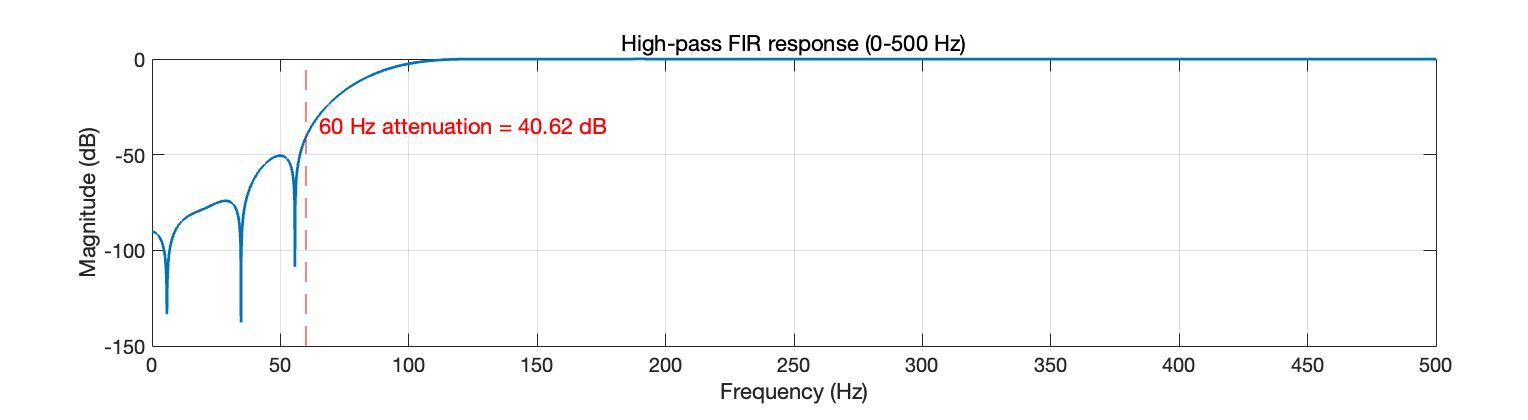
\includegraphics[width=0.72\textwidth]{figures/fig15.png}
    \caption{Problem 3 滤波器设计参数与频响界面}
\end{figure}

\subsection{量化结果与验证}
\begin{figure}[H]
    \centering
    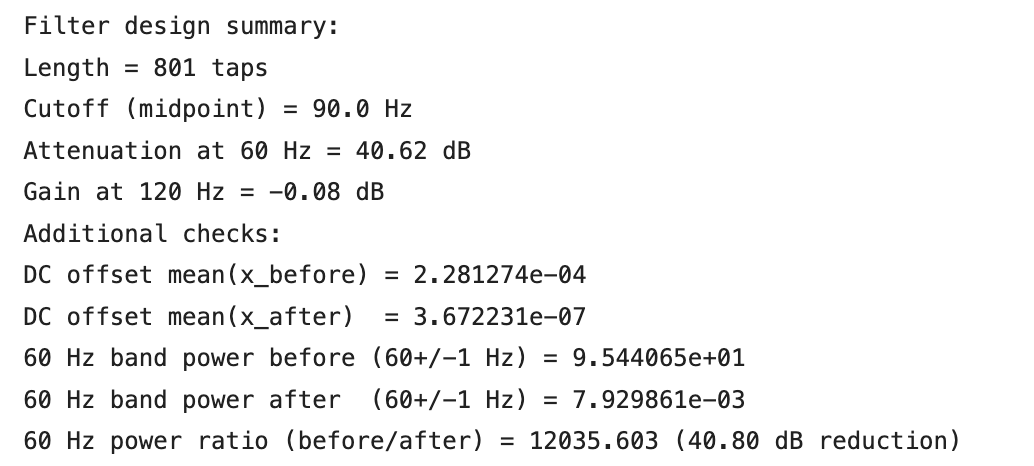
\includegraphics[width=0.86\textwidth]{figures/fig16.png}
    \caption{MATLAB 文本输出：滤波器指标与附加检查结果}
\end{figure}

核心数值如下：
\begin{itemize}
    \item 滤波器长度：801 taps
    \item \SI{60}{Hz} 衰减：\SI{40.62}{dB}
    \item \SI{120}{Hz} 增益：\SI{-0.08}{dB}
    \item DC offset：\(\mathrm{mean}(x_{before})=2.281274\times10^{-4}\)，\(\mathrm{mean}(x_{after})=3.672231\times10^{-7}\)
    \item \SI{60\pm1}{Hz} 窄带功率下降：\SI{40.80}{dB}
\end{itemize}

\begin{figure}[H]
    \centering
    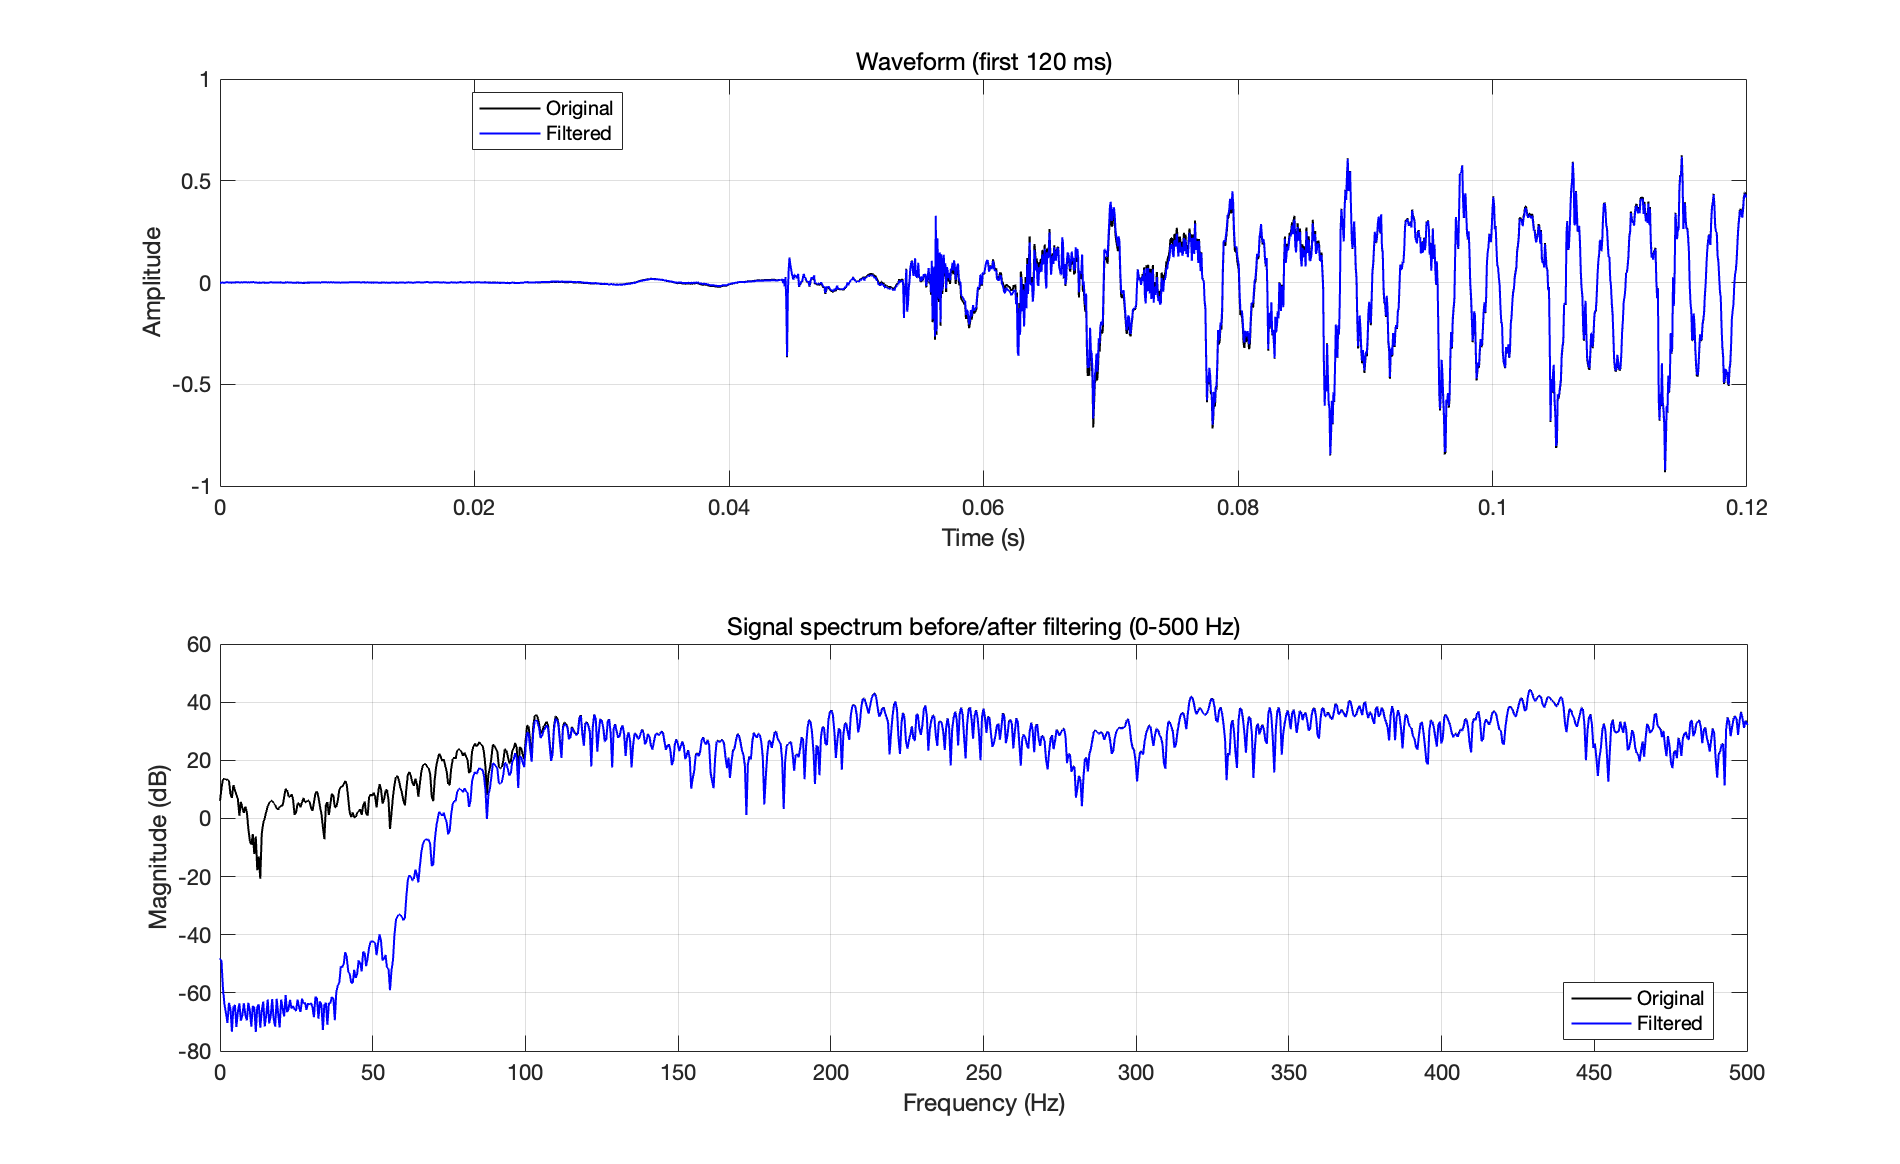
\includegraphics[width=0.88\textwidth]{figures/fig17.png}
    \caption{滤波前后波形与低频频谱对比}
\end{figure}

结论：理论频响和实测窄带功率均满足 \SI{60}{Hz} 至少 \SI{40}{dB} 衰减要求。

\subsection{输出文件}
生成新文件：\texttt{test\_16k\_hp.wav}。

\subsection{关键代码段}
\begin{lstlisting}[caption={Problem 3 FIR 高通滤波设计与滤波执行}]
fStop = 60;
fPass = 120;
targetAtt60 = 40;
[b, report] = designHighpassFIR(fs, fStop, fPass, targetAtt60);

yFilt = conv(x, b, 'same');
peak = max(abs(yFilt));
if peak > 0.999
    yFilt = 0.999 * yFilt / peak;
end
audiowrite('test_16k_hp.wav', yFilt, fs);
\end{lstlisting}

\begin{lstlisting}[caption={Problem 3 DC 偏置与 60Hz 功率比验证}]
meanBefore = mean(x);
meanAfter = mean(yFilt);

p60Before = bandPowerAroundFreq(x, fs, 60, 1);
p60After  = bandPowerAroundFreq(yFilt, fs, 60, 1);
ratio60 = p60Before / (p60After + eps);
ratio60dB = 10 * log10(ratio60 + eps);

fprintf('DC offset mean(x_before) = %.6e\n', meanBefore);
fprintf('DC offset mean(x_after)  = %.6e\n', meanAfter);
fprintf('60 Hz power ratio (before/after) = %.3f (%.2f dB reduction)\n', ...
    ratio60, ratio60dB);
\end{lstlisting}

\section{全实验结论}
本次实验完整完成 Problem 1--3 全部要求，主要结论如下：
\begin{enumerate}
    \item Problem 1：完成 ARPAbet 转写、句子分段标注、元音/辅音置零处理与可懂度比较。结果表明在该句中辅音对词汇区分的贡献更显著。
    \item Problem 2：完成 MATLAB 与 Praat 双路径 Formant 提取。实测值与理论均值存在系统偏差，但三元音相对分布关系与理论一致，元音类别识别有效。
    \item Problem 3：完成线性相位 FIR 高通滤波设计与验证，\SI{60}{Hz} 抑制达到题目要求（理论 \SI{40.62}{dB}，实测 \SI{40.80}{dB}），并输出新音频文件。
\end{enumerate}


\ifPDFTeX\end{CJK*}\fi
\end{document}
